\chapter{Introduction and Background}

\section{Introduction}

The human body is a four-billion-year-old piling-up of nanotechnological hacks, which exists because, for that four billion years, none of its ancestors died without issue; we have hijacked it and are now attempting to use it for our own ends. We don't know how it works, and we don't have the servicing equipment to fix it when it breaks. The goal of human genomics is to figure out how our bodies actually work, so that we can do more than change the nanotechnological oil.

Achieving this goal is relatively difficult, because of the scale of the problem. Each human genome is about 3.2~billion base pairs, and each human has two genomes (one from each gamete). %Each of those base pairs has four possible values (\texttt{A}, \texttt{C}, \texttt{G}, \texttt{T}), providing a truly untennable $3.16 \times 10^{3853183944}$ combinations.
Human brains struggle to think about a even a single billion of anything, a number so large that a one-in-a-million chance occurs on average a thousand times. Add to this the already-difficult-to-comprehend non-designed-ness of the entire system, where no part is ``for'' anything, and you can begin to get a sense of the difficulty of the problem.

Fortunately, despite our limitations, we are beginning to develop techniques and guiding principles for working with problems at these scales. One of those principles is that large problems can be effectively addressed by integrating across large data sets~\cite{halevy2009unreasonable}. With a population now exceeding 7.5~billion individuals, humans may constitute a sufficiently large data set to begin to approach this problem~\cite{talton2017economics}. However, effective tools to use genomic information at the scale of the human population will be required.

Human genomics as it exists today is organized around something referred to as ``the human genome'', obtained at great expense through the Human Genome Project~\cite{powledge2003human}. There is a clear distinction in the field between the human genome, embodied by the \vocab{primary assembly} in reference genome assembly builds produced by the Genome Reference Consortium (GRC)~\cite{schneider2013genome}, and databases of genomic variation, such as the variant sets produced by the 1000 Genomes Project~\cite{10002015global} or the Simons Genome diversity Project~\cite{simons2014simons,simons2017simons}. Such efforts generally distribute variation information in Variant Call Format (VCF) files, which present the data in the coordinate space defined by the GRC's assembly. Actual sequencing data is presented in Binary Alignment/Map (BAM) files, which give each sequencing read's alignment to the GRC's assembly. This linear coordinate system, which refers to locations in peoples' genomes by the chromosome and base index in the primary assembly, is the foundation of genomics.

Unfortunately, this approach will not scale, because as our view of the human population becomes wider, our view of human genomic variation is also broadening. The most recent release of the GRC's human reference genome assembly, GRCh38, contains 261 \vocab{alternate (alt) loci}~\cite{grc2013announcing}, up from a mere nine in the previous assembly~\cite{grc2009grch37}. Alternate loci are sequences intended to provide alternative versions of parts of other sequences in the primary assembly, in order to be more representative of large-scale and structural variation in the human population~\cite{karolchik2014new}. When analyzing or describing a sample with a haplotype closer to one of the alt loci than to the corresponding primary assembly region, that alt locus can be used to fulfill the functions of a reference sequence for that region, replacing part of the primary assembly sequence. The number of genomes for which this replacement ought to be performed is relatively large. A recent study~\cite{jager2016alternate} found that some alternate loci are likely to be present in 90\% or more of the individuals in some populations. The eight alternate loci for the Major Histocompatibility Complex (MHC) region were chosen to be representative of people of European ancestry~\cite{horton2008variation}; many analyses of the genomes of people of European ancestry might benefit from using one of those alternate loci in place of what is in the primary assembly. However, available variation data sets~\cite{10002015global}, and indeed the VCF format itself~\cite{danecek2011variant,marshall2013variant}, do not allow for this, and instead cram all individuals into the space of the primary assembly, regardless of its appropriateness for the individuals or populations under study. On the software side, alternate loci support is still a novelty~\cite{jager2016alternate}.

% Can I find a source saying that this proliferation of alt loci is unexpected?

In genomic regions where these alternate loci apply, the traditional, primary-assembly-based linear coordinate system begins to break down. To properly reason about such genomic regions, we need to abandon either the idea that bases in peoples' genomes correspond to bases in a reference, or the idea that references are linear. Whereas in the previous assembly the problem was relatively contained, in GRCh38 this sudden proliferation of alternate loci is poking holes in that abstraction all over the genome, making the problem much more urgent.

% TODO: Cut this? I didn't really do anything with it. Maybe the existence of centromeres should be background?
The linear organization of the reference genome also frustrates attempts to study regions of the genome which are difficult to assemble, or which, due to sequence similarity, are very difficult to distinguish from similar regions at other locations in the genome. To facilitate analysis of the centromeres, for example, GRCh38 includes plausible synthetic linear centromere sequences~\cite{karolchik2014new}. We have more precise, graph-based models of what we actually know about the centromeres, but these models cannot be indexed by linear sequence coordinates or processed by tools that expect a linear reference sequence~\cite{miga2014centromere}.

\begin{sloppypar}
I propose a nonlinear, graph-based ``Human Genome Variation Map'', or HGVM. This new type of genomic reference will eliminate the artificial distinction between the reference genome assembly---``the human genome''---and what we know about variation among the genomes of the human population. A graph-based reference can capture in a first-class way the sequence information which is currently relegated to alt loci, as well as additional variant information from sources like the 1000 Genomes Project~\cite{10002015global}. If it managed to avoid giving preference to one version of a region with alternate loci over another, a human genome variation map could potentially combat \vocab{reference (allele mapping) bias}, an effect in which alleles that match a single linear reference are easier to detect than those which do not~\cite{degner2009effect,brandt2015mapping}. The adoption of a unified representation of genomes will allow genomic analysis software to scale to much larger cross-dataset analyses, with a more representative view of individuals' genomes, allowing progress to be made in the unraveling of human biology.
\end{sloppypar}

\section{Background}

\subsection{How Genomics Works}

The human reference genome assembly was built at great expense at the turn of the millennium and is maintained by the Genome Reference Consortium (GRC)~\cite{church2011modernizing}. This reference genome assembly was originally created by stitching together actual observed pieces of DNA sequence into a single-copy haploid \vocab{golden path} representing a complete genome~\cite{church2011modernizing}. Under this model, a hypothetical perfect assembly would have a single \vocab{contig}, or contiguous linear string of DNA bases, per chromosome. This naturally suggests a coordinate system: bases can be referred to by the contig they are on and their offset from the beginning of that contig.

This coordinate system is a critical piece of genomics infrastructure. It allows the reference genome to be annotated with genes and other elements. It provides the backbone to which descriptions of genomic variation are anchored. It defines the space in which genome sequencing happens, as short reads from sequencing machines are \vocab{mapped} to positions in this space. The entire field depends on this coordinate system.

Unfortunately, whenever the official human reference genome is updated, and bases are inserted or removed, the old coordinates are no longer valid on the new reference, and a period of mass confusion ensues as everyone who studies human genomics translates everything they are working on over to the new coordinate system, and then wonders whether their colleagues have done the same. Resources that aren't converted to the new system are at best lost to the field, and at worst applied inappropriately to the wrong genomic locations.

The golden path model is inextricably bound to the concept of ``the human genome''---the idea that one prototypical set of 24 chromosomes is a suitable foundation for the field of genomics. This idea has been central to human genomics, but it is not without its flaws. Putting aside the unfortunate normative implications of declaring the allele from whomever you sequenced first as ``reference'' and any alternatives from other populations as ``variant'', using a single reference genome when mapping sequencing reads leads to the well-known phenomenon of reference bias~\cite{degner2009effect,brandt2015mapping}. Reads matching the reference genome at a variant site tend to map better and more often than those supporting differences from the reference. This reference bias affects many popular short-read aligners~\cite{lunter2011stampy}. Additionally, in some genomic regions there are dramatically structurally distinct haplotypes present in the population~\cite{church2011modernizing}. One example of this phenomenon is the extremely variable Major Histocompatibility Complex (MHC) region on chromosome 6. Mapping reads only against the single haplotype actually included in the assembled golden path will almost certainly make it harder to map reads from other haplotypes.

% TODO: resolve golden path, primary path, primary reference, etc. which all sort of mean the same thing.
% Also explain contig vs. scaffold.

\subsection{The Release of GRCh38}

A new version of the official human reference genome, GRCh38, was released in 2013~\cite{grc2013announcing}. In addition to marking the transition to a unified version numbering scheme across major genome browsers, this new release continues the GRC's gradual migration away from the golden path concept. Although GRCh38 is still constructed around a single (chimeric) haploid genome, the new reference assembly also provides sequences for hundreds of so-called \vocab{alt loci}---additional pieces of sequence with a specified alignment to that genome which describe some of the structurally distinct local genomic arrangements which have been observed in humans. The older GRCh37, by comparison, contained only three genomic regions with alt loci~\cite{church2011modernizing}. This means that the GRCh38 assembly, taken as a whole, is fundamentally nonlinear at more than just a few problematic locations. Unfortunately, popular tools like BWA, being originally designed for aligning to a single-copy primary assembly, need to apply complex heuristics to account for these alt loci~\cite{li2014bwa,li2014new}.

The new assembly also contains sequence for the centromeres---the central portions of the chromosomes, which contain extremely repetitive sequences that continue to defy conventional sequencing and assembly methods~\cite{karolchik2014new}. However, these new centromere sequences are not directly derived from actual sequence observations, but are instead plausible linearizations of a series of graph-based centromere models~\cite{miga2014centromere}. Unfortunately, the linear format discards much of the uncertainty information present in the graph models. Moreover, this additional sequence was found during testing to cause trouble for traditional short-read alignment pipelines, so GRCh38 also comes as an ``analysis set'' with these sequences masked out~\cite{karolchik2014new}. The real problem, though, lies with the tools, which cannot handle either a full nonlinear description of what we know about the centromeres or even the placeholder linearization that GRCh38 includes.
% TODO: Cut this paragraph since I don't really solve this problem?

In summary, GRCh38 marks the continuation of a trend towards nonlinearity in the human reference and provides an example of the shortcomings of the golden path approach. Until tools can be updated to account for alt loci and centromere sequences, GRCh38 cannot be used to its full potential.

\subsection{The Genome Reference Consortium Assembly Model}

% Here is actually how the GRC represents the assembly
    % It is not quite just a linear thing
    
Containing as it does both the golden-path-style assembled primary chromosomes and an increasing number of alternate loci, the GRC's human genome assembly needs to have a formally organized structure. The assembly is broken down into \vocab{units}, each of which contains a set of \vocab{sequences}~\cite{schneider2013genome}. The most important unit is the \vocab{primary assembly unit}, which is also referred to as the ``primary assembly'' or ``primary path''. This unit contains the full-chromosome sequences for all of the human chromosomes (1-22, X, and Y), as well as \vocab{unplaced scaffolds}, which are pieces of DNA that are thought to be chromosomal but have not yet been associated with a chromosome, and \vocab{unlocalized scaffolds}, which are associated with a chromosome but have not been inserted into that chromosome's sequence~\cite{schneider2013genome}. The point of the primary assembly unit is to be a complete haploid genome, containing exactly one version of every component~\cite{schneider2013genome}. (Note, however, that mitochondrial DNA is relegated to its own \vocab{non-nuclear assembly unit}.)

The alternate loci are layered on top of the primary assembly unit in a series of \vocab{alternate loci assembly units}~\cite{schneider2013genome}, which are numbered (\texttt{ALT\_REF\_LOCI\_1}, \texttt{ALT\_REF\_LOCI\_2}, ...). Each alternate loci assembly unit contains at most one alternate locus for each genomic region having alternate loci. This means that the first alternate loci assembly unit will have the most alternate loci in it, and later units will have fewer, with the total number of units being the same as the number of alternate loci for the region that has the most alternate loci (which, in GRCh38, is the LRC\_KIR region)~\cite{grc2013announcing,schneider2013genome}. This data model is designed to be able to represent distinct, linked haplotypes, as is done in the GRC mouse assembly, but for human this capability is not used, and so no significance is assigned to two alternate loci being in the same assembly unit~\cite{schneider2013genome}.

Finally, as an attempt to work around the disruptive impact of new assembly releases with changed coordinate systems, the GRC assembly model includes a \vocab{patches assembly unit}, containing \vocab{patch scaffold} sequences~\cite{schneider2013genome}. The patches are divided into two types: \vocab{fix patches}, which are intended to replace an erroneous part of a sequence from another assembly unit with an improved, corrected sequence, and \vocab{novel patches}, which represent new alternate loci~\cite{schneider2013genome}. The GRC uses this patch model so that the coordinates of the other assembly units can be preserved (avoiding disruption and maintaining backward compatibility with existing annotations) while still allowing new alt loci or corrections to existing sequence to be rolled out in a timely fashion (i.e. once per quarter, rather than once every few years)~\cite{schneider2013genome}.

The regions to which alternate loci belong, and official GRC alignments of the alternate loci to the portions of the primary assembly unit that they are intended to replace, are also part of the assembly model~\cite{schneider2013genome}. The region definition mechanism is also used to model the pseudoautosomal regions of the X and Y chromosomes~\cite{schneider2013genome}.
    
\subsection{Modeling Human Genomic Variants with VCF}

Unlike in the assembly world, the world of human variation data is more fractured. One particularly large database is dbSNP~\cite{sherry2001dbsnp}, but it works at the level of the individual variant. There is also the variation data maintained by the GRC, in the form of alternate loci. However, the most influential institution in the study of human genomic variation so far has been the 1000~Genomes Project. The 1000~Genomes Project maintains and distributes variant data for over 2,500 people's genomes~\cite{sudmant2015integrated}. However, their greatest contribution to the field may be the development of the extremely popular \vocab{Variant Call Format} (VCF), a column-based text file format used to represent variation data, now maintained by the Global Alliance for Genomics and Health~\cite{danecek2011variant}. Samples are represented by columns, and polymorphic positions in the human genome by rows. VCF files can be supplemented by an index on genomic position, but no work appears to have yet been done to also provide an index by sample; consequently, the scalability of VCF is currently limited to numbers of samples that can be scanned through efficiently~\cite{danecek2011variant}. Moreover, being primarily about a file format instead of a conceptual data model, the VCF specification~\cite{marshall2013variant} primarily discusses syntactic considerations, rather than semantic or pragmatic concerns.

VCF encodes individual samples' genomes by defining a series of variant sites along the length of the linear reference genome, defining a set of alternate alleles which have been observed at each site (in addition to the allele in the reference), and then indicating which alleles (in what phasing) are present in each sample at each site. This approach works extremely well for some types of variation, like single nucleotide polymorphisms (SNPs) and short indels in structurally quiet regions, but it also has shortcomings.

One problem with the VCF format is it does not define the semantics of the absence of a variant record. Does it mean that that position in the reference is known not to be variable in the population (or at least in the sampled portion of it)? Or does it mean that that location is not in the region covered by the VCF file? To solve this problem, the VCF format has been extended by Illumina to create the gVCF format, in which genotyped but nonvariant positions are also described~\cite{saunders2014about}.

Another potential problem with the VCF format, at least from the point of view of people who need to read it, is that it is very featureful. The format is extensible, through the inclusion of header lines defining various fields. However, different VCF processing tools need to have different sets of fields defined in order to work, and some tools or data sets \cite{sudmant2015integrated} will use extra fields to modify the interpretation of standard fields defined in the VCF specification~\cite{marshall2013variant}. To avoid crashes and to ensure that variant calls are interpreted as the caller intended, it is vital to check the fields output by one tool against those accepted by another. This makes VCF a worse standard, because any two tools that both use VCF cannot necessarily communicate with each other, and because communication failures can be silent if the two tools agree mostly but not perfectly.

Furthermore, there are no fewer than three distinct syntaxes for specifying variants in VCF: the original syntax, in which alternate alleles are short stretches of sequence; a symbolic format, in which alternate alleles are mere specifications of inversion or duplication, or even references to named alleles defined elsewhere; and a breakend-based format, in which structural variants (and related sequence changes) are defined as a series of possibly-paired breakend records describing how the reference would have had to have been cut and spliced to produce the sample~\cite{marshall2013variant}. Available VCF parsers do not help with integrating across or converting between these different internal formats, and some don't even support all of them. Tools written to directly extract information from VCFs without a parser library often support only one or maybe two of these formats. Between the three different formats and the fact that different alignment parameters can induce variant callers to describe the same observed sequence as different variants, it is very difficult to compare two VCF files.

Finally, the VCF format is tightly coupled to the linearity of the reference genome assembly. While VCF's breakend system allows the specification of complex rearrangement graphs for samples, there is no explicit support for even the alt loci of the current GRCh38 reference. For example, if one were to specify variant records on one of the MHC alt loci, there would be no way to specify phasing with respect to variants on the main chromosome 6, because VCF specifies records with different chromosome names to be unphased relative to each other~\cite{marshall2013variant}. Furthermore, there is no way to explicitly specify that a sample uses a certain alt locus; it would be necessary to infer this from the existence of called genotypes in the coordinates of that alt. It would certainly be possible to adopt certain conventions within the existing VCF format to work around this problem---for example, we could wire the alt loci into their parent chromosomes with breakends whenever they are present. However, no such conventions are standardized for data interchange.

A graph-based approach to the description of genomic variants could alleviate several of these problems, defining explicitly when an individual matches the primary assembly, and expressing clearly and concisely the alt loci that an individual carries, and any variations on top of them, in a single sufficiently general syntax.

\subsection{The 1000 Genomes Project}

Besides the development of the VCF standard, the 1000~Genomes Project has also conducted one of the most useful publicly available surveys of human genomic variation to date~\cite{10002015global}. The 1000 Genomes Project data set is more consistently collected and analyzed than data from the Personal Genome Project (PGP)~\cite{church2005personal}. It is also easier to download than the Simons Genome Diversity Project dataset~\cite{simons2017simons}, requiring neither special software nor manual approval. For these reasons, the 1000 Genomes Project dataset is the standard human variation dataset to use in analyses.

The dataset contains genomes from 2,504~people across five \vocab{superpopulations} and 26 populations~\cite{10002015global}, as shown in Table~\ref{tbl:populations}. Sample collection goals and informed consent practices were broadly similar to those developed for the HapMap project, from which some of the initial samples were obtained~\cite{international2004integrating}. In particular, the seductiveness of the three-letter-code abstraction notwithstanding, the goal is not to build a system or hierarchy of racial or ethnic categories for dividing up the human population~\cite{international2004integrating}. Rather, the avowed intention is to describe where and from whom sample DNA was collected, although this necessarily relies on an implicit system of racial and ethnic categories.

\begin{table}
\centering
\begin{tabular}{llp{6cm}}
\textbf{Superpopulation} & \textbf{Population} & \textbf{Provided Description} \\
\hline
AFR & ESN & ``Esan in Nigeria'' \\
& GWD & ``Gambian in Western Division, Mandinka'' \\
& LWK & ``Luhya in Webuye, Kenya'' \\
& MSL & ``Mende in Sierra Leone'' \\
& YRI & ``Yoruba in Ibadan, Nigeria'' \\
& ACB & ``African Caribbean in Barbados'' \\
& ASW & ``People with African Ancestry in Southwest USA'' \\
\hline
AMR & CLM & Colombians in Medellin, Colombia'' \\
& MXL & ``People with Mexican Ancestry in Los Angeles, CA, USA'' \\
& PEL & ``Peruvians in Lima, Peru'' \\
& PUR & ``Puerto Ricans in Puerto Rico'' \\
\hline
EAS & CDX & Chinese Dai in Xishuangbanna, China'' \\
& CHB & ``Han Chinese in Beijing, China'' \\
& CHS & ``Southern Han Chinese'' \\
& JPT & ``Japanese in Tokyo, Japan'' \\
& KHV & ``Kinh in Ho Chi Minh City, Vietnam'' \\
\hline
EUR & CEU & Utah residents (CEPH) with Northern and Western European ancestry'' \\
& GBR & ``British in England and Scotland'' \\
& FIN & ``Finnish in Finland'' \\
& IBS & ``Iberian Populations in Spain'' \\
& TSI & ``Toscani in Italia'' \\
\hline
SAS & BEB & Bengali in Bangladesh'' \\
& GIH & ``Gujarati Indians in Houston, TX, USA'' \\
& ITU & ``Indian Telugu in the UK'' \\
& PJL & ``Punjabi in Lahore, Pakistan'' \\
& STU & ``Sri Lankan Tamil in the UK'' \\
\hline
\end{tabular}
\caption[Populations and superpopulations from the 1000 Genomes Project]{Populations and superpopulations from the 1000 Genomes Project~\cite{10002015global}.}
\label{tbl:populations}
\end{table}

\subsection{Substring Search with the Suffix Array}

The \vocab{suffix array} of a string is an array of indices into the string, sorted in the lexicographical order of the suffixes that they point to~\cite{manber1993suffix}. For example, the string ``dog'' has suffixes ``dog'' at index 0, ``og'' at index 1, and ``g'' at index 2, so its suffix array would be $[0, 2, 1]$, corresponding to the suffix sort order $[\textrm{``dog''}, \textrm{``g''}, \textrm{``og''}]$. Another example suffix array for the string ``GATTACA'' is visible in the leftmost column of Figure~\ref{fig:bwt}.

Suffix arrays have some useful properties. Most importantly, all of the suffixes that start with the same substring appear in a single contiguous block~\cite{ferragina2000opportunistic}. This block starts at the position corresponding to the number of occurrences of lexicographically smaller substrings of the same length~\cite{ferragina2000opportunistic}. This is particularly obvious in the case of single-character substrings: all the suffixes (and, thus, all the substrings) beginning with a certain character appear in one block, coming immediately after all suffixes beginning with lexicographically smaller characters.

Suffix arrays can be used as indices to speed up substring search on the string they are derived from. Because of the block structure described above, and because every instance of a substring is at the beginning of some suffix, a simple binary search is sufficient to find any substring that is present, and a scanning up and down from one instance can pull out the entire corresponding block~\cite{manber1993suffix}. Supplementing the suffix array with a \vocab{longest common prefix (LCP)} array, holding the length of the prefix shared by each pair of adjacent suffixes, can further speed up the search, by requiring only a single-character comparison (instead of a string comparison) at each search step~\cite{manber1993suffix}.

\subsection{String Compression with the Burrows-Wheeler Transform}
\label{subsec:bwt}

Human genomes, being extremely similar to each other and relatively similar to themselves in different places, lend themselves to compression. One particularly useful algorithm in string compression is the \vocab{Burrows-Wheeler Transform (BWT)}. The BWT takes strings and rearranges them for increased compressibility, by putting characters from similar contexts near each other~\cite{burrows1994block}. (It is interesting to think of the BWT as defining a new, context-based coordinate system.)

The BWT operates by taking the string to be compressed (with a sentinel value ``\$'' lexicographically smaller than all other characters appended to it) and imagining all possible rotations of it~\cite{burrows1994block, ferragina2000opportunistic}. Each rotation is derived from the previous one by taking the first character and moving it to the end~\cite{burrows1994block}. The rotations are then sorted lexicographically, and the last characters of all the rotations become the transformed string~\cite{burrows1994block}.

The BWT makes strings more compressible by grouping characters by the contexts they appear in (specifically, the strings they appear before). If two characters both appear before a suffix starting with ``andy'', they will appear near each other in the BWT. Assuming some letters are more likely, relative to the overall frequency distribution, to precede this string than others are (for example, ``c'' and ``h'' as opposed to ``e'' or ``n''), this creates a region of the BWT which is enriched for those characters. This enrichment makes the region more compressible by move-to-front or even simple run-length encoding~\cite{burrows1994block}.

The implied BWT matrix, with all the sorted rotations as rows, is generally not kept, but it is often useful to consider the BWT string in its context as the last column of that matrix~\cite{burrows1994block, ferragina2000opportunistic}. It is also useful to think of this matrix as being made up of ``character instances''; characters in the matrix that are derived from the same position in the original string are the same character instance. (Imagine uniquely numbering the character at each position on the original string before creating the matrix.) Such a matrix is visible in Figure~\ref{fig:bwt}.

\begin{figure}[ht]
    \centering
    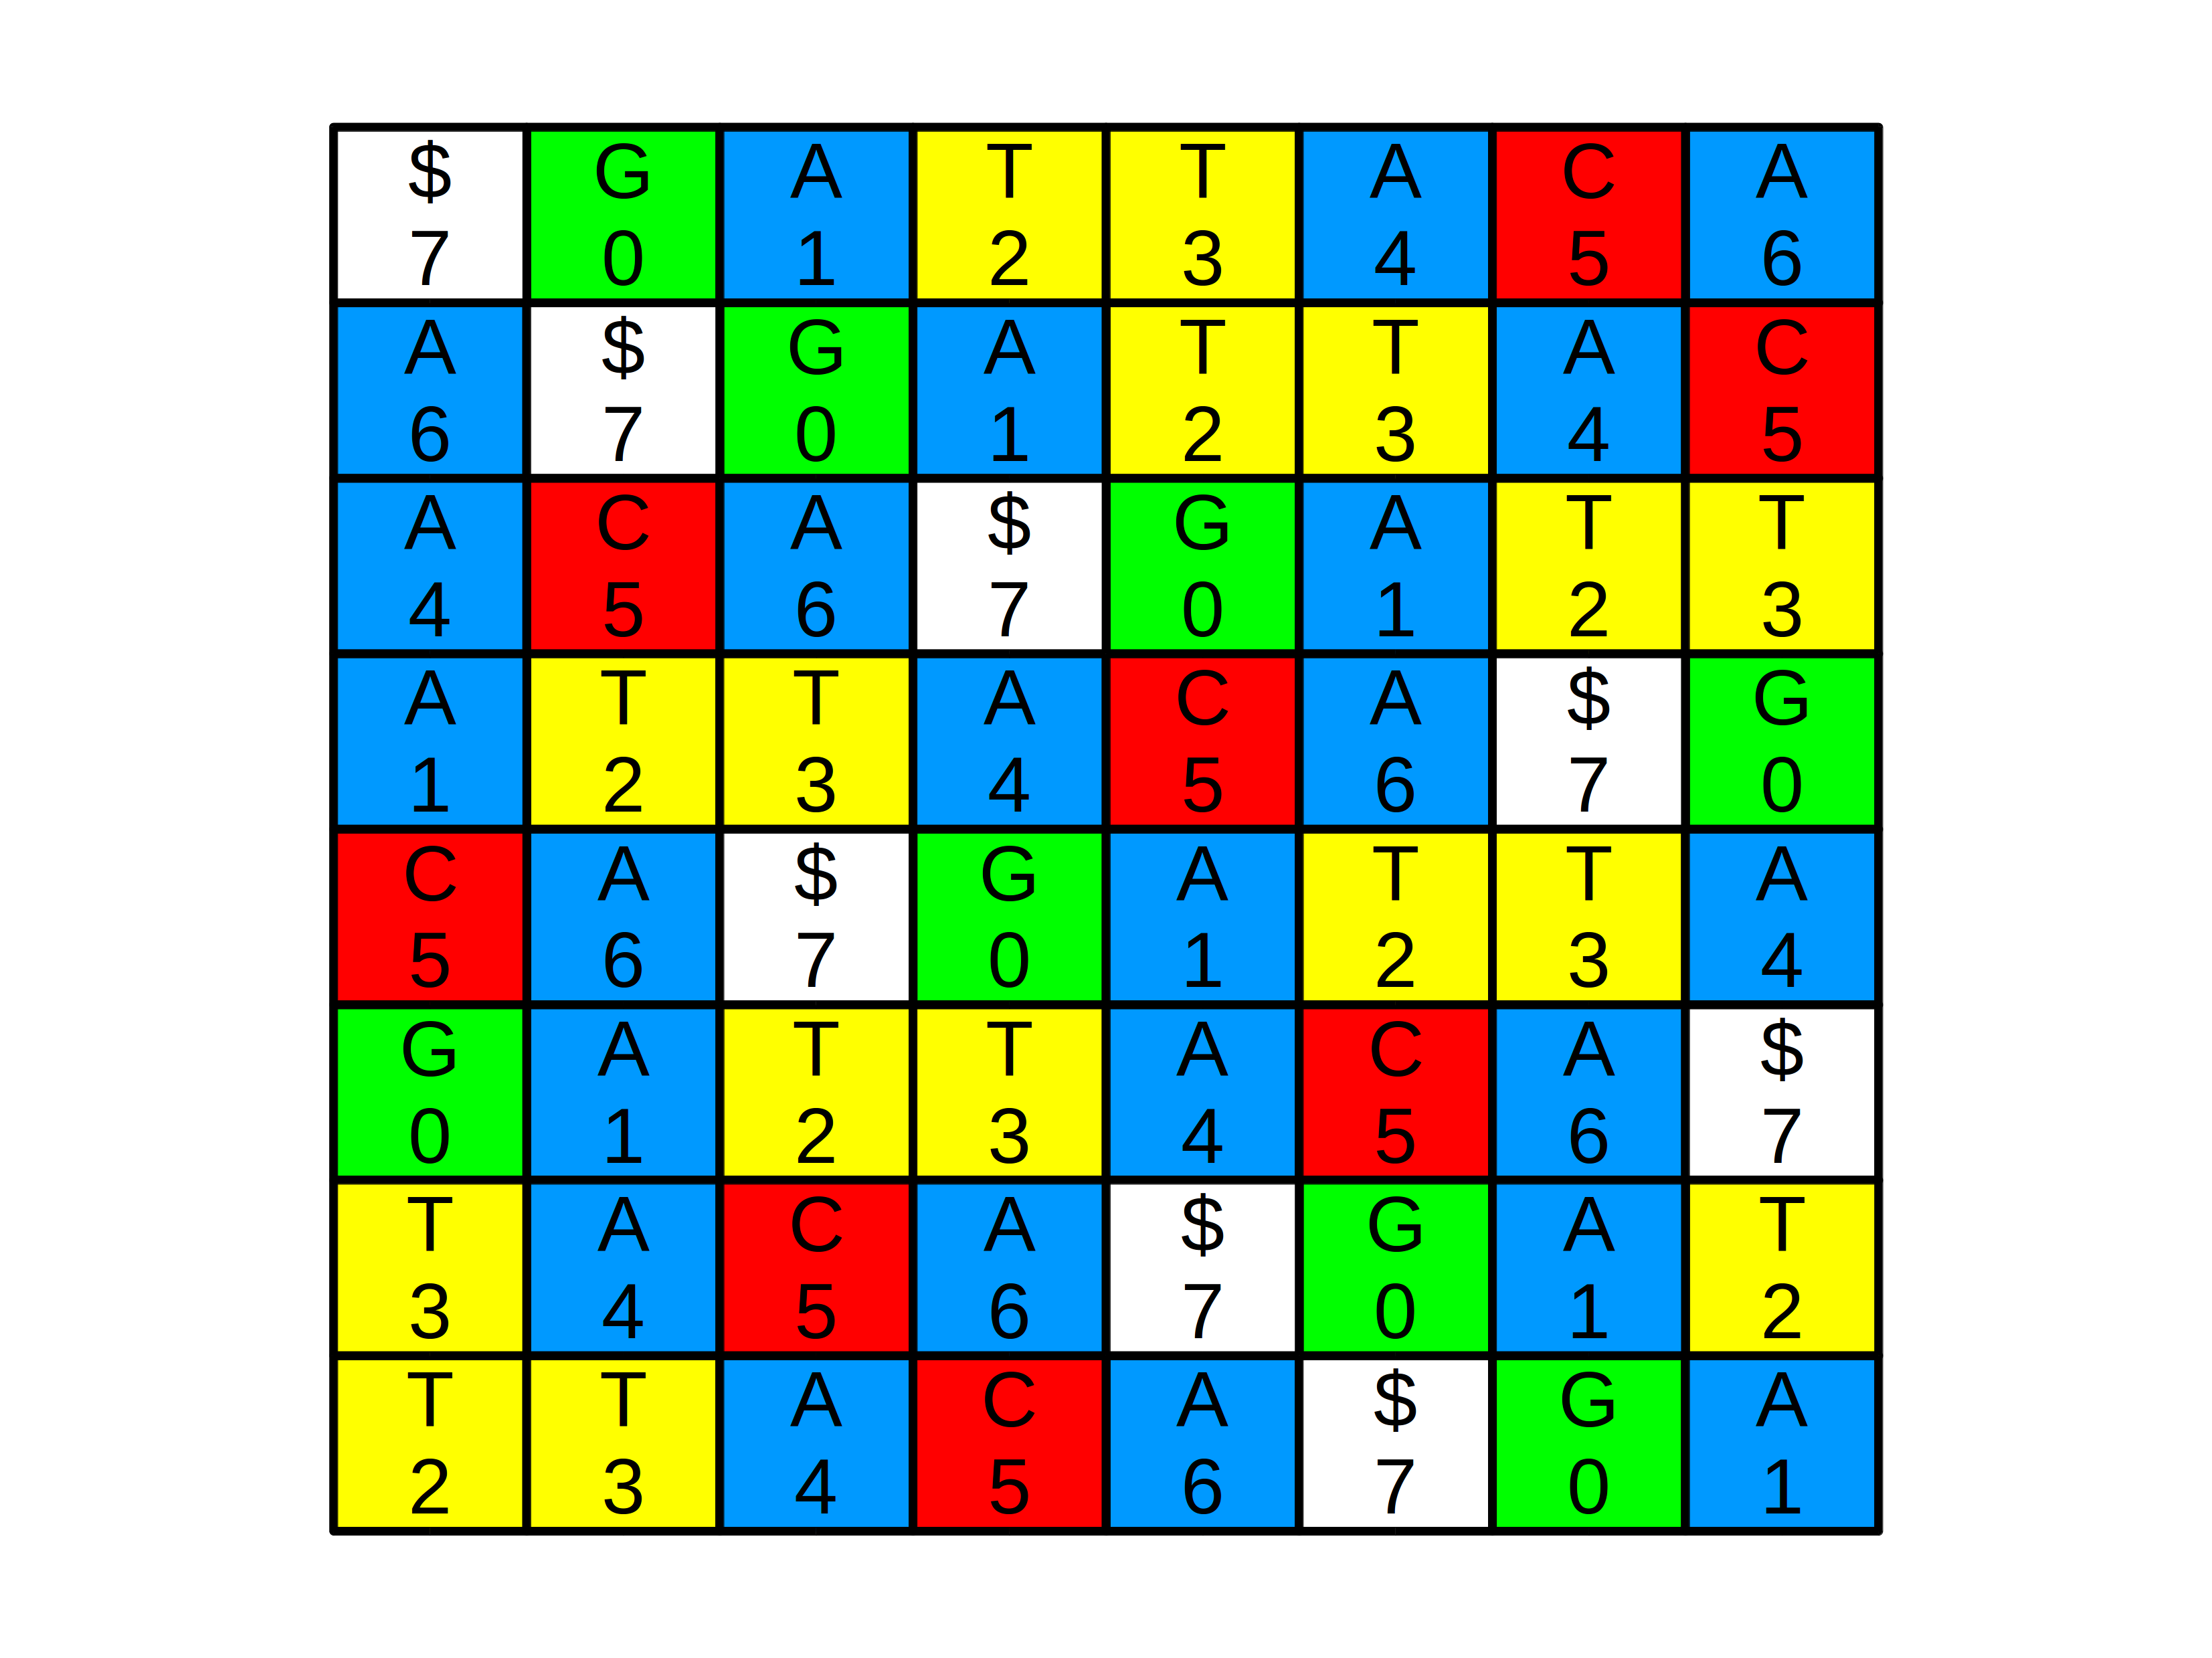
\includegraphics[width=1.0\textwidth]{figures/01_introduction/bwt.png}
    \caption[An example BWT matrix for the string ``GATTACA'']{An example BWT matrix for the string ``GATTACA''. The sentinel value ``\$'' is appended to the end of the string, all rotations of the string are calculated, and the rotations are sorted. Bases are colored according to base identity and numbered according to position in the original string. The characters in the far right column are the BWT of the original string, while the numbers in the far left column are the suffix array (represented as indices into the original string).}
    \label{fig:bwt}
\end{figure}

We can show that, for each character in the alphabet, corresponding instances of that character will appear in the same order in the first column and in the last column. Consider just the rows where the character in question appears in the first column. When sorting these rows, the first column is uninformative (since it is constant across all rows), and the rows are sorted lexicographically by the remaining columns in order. Rotating all the strings so the uninformative column appears last will not change the order of the other columns, and thus will not change the relative sort order of the rows we are considering. Thus the instances of the character stay in the same relative order in the last column as in the first column~\cite{langmead2013introduction}.
    
\subsection{Searching in BWTs with the FM-index}

Constructing the BWT matrix is essentially the same task as constructing the suffix array of the string being transformed. All the rotations of the string contain the ``\$'' sentinel which is lexicographically less than all other characters. Thus the rotations are actually sorted by the portion before the ``\$'' character---that is, by the corresponding suffixes of the original string. This is the same sort used to construct the suffix array.

A BWT can be augmented with a small amount of additional information to create an \vocab{FM-index} (named after the initials of its inventors), which, like a suffix array, allows efficient substring search on the original string, but which also retains the compression afforded by the BWT~\cite{ferragina2000opportunistic}. The FM-index is based primarily on the idea of a \vocab{last-first (LF)} mapping. This mapping maps each character instance in the last column of the BWT matrix to the row in which that same character instance appears in the first column. Because each BWT matrix row is a rotation of the original string, the last column of the row will contain the character instance immediately preceding the one just looked up. Thus, following the LF-mapping around the BWT from any starting position allows the characters of the original string to be enumerated from there in reverse order~\cite{ferragina2000opportunistic}.

Since only the last column of the BWT matrix (i.e. the actual BWT string) is used in the algorithm, only that string needs to be stored. Furthermore, the LF-mapping can easily be calculated from the BWT string. To LF-map the character instance at a certain index in the BWT, count up the number of characters in the BWT lexicographically less than the character, and add the character instance's rank among all instances of that character. This gives the index of the LF-mapping result in the BWT.

To see why this works, recall that in a suffix array, and thus also in the BWT matrix, all the suffixes (or here rotations) that start with a given character form a contiguous block, coming just after all those beginning with smaller characters. Thus, the first calculation is to find the start of this block. And since, as shown in Subsection~\ref{subsec:bwt}, the relative order of character instances in the first column is the same as that in the last column, to find the offset of this particular character instance in that contiguous block, we merely need to find its rank among instances of the same character in the last column, which is the BWT string~\cite{langmead2013introduction}.

We can now define \vocab{backward search}, a search algorithm using the BWT which processes the characters in the query string from back to front. The algorithm begins by selecting the entire BWT matrix, which is the range of suffixes that begin with the empty string. Then, for each character in the query string, from the last forwards, the algorithm extends the searched string at the front with that character. It takes the new character and finds the first and last instances of it in the BWT contained within the currently selected result range. It then LF-maps each of those instances, and takes the range between them as the new result range for the query string extended with that character. If there are no instances of the character to map, then the searched string is not found in the index~\cite{ferragina2000opportunistic}.

Each row of the BWT matrix in the old range started with an instance of the old query string. Each of the rows that ended in the new query character corresponded to an instance of the old query string occurring after the new query character, and thus each implies an instance of the new, one-character-longer query string. The LF-mapping step finds the contiguous block of rows in the BWT matrix where those instances of the search string appear, the boundaries of which correspond to the first and last instances of the new character in the old BWT range (by the conservation of ordering mentioned at the end of Subsection~\ref{subsec:bwt}). Thus, such an algorithm can be used to search for substrings in a string, using the BWT of the string~\cite{ferragina2000opportunistic}.

By pre-calculating some auxiliary data structures, such as a table with the start index of each character's range in the BWT matrix, and by using succinct data structures for $O(1)$ rank queries, this algorithm can be made to run in time linear in the length of the query string, and constant in the length of the index~\cite{ferragina2000opportunistic}. Furthermore, using a downsampled copy of the suffix array, the location of each result in its source string can be calculated efficiently~\cite{siren2009run}.

\subsection{Bidirectional DNA Search with the FMD-Index}

BWT-based indices have found many applications in genomics, mostly due to their ability to efficiently search for and identify the locations of a substrings in very large data sets---with a few modifications, this search can be extended to align reads to a reference~\cite{li2014bwa}. The popular short read aligner BWA, for example, is built on an FM-index of the reference genome; indeed, the name stands for ``Burrows--Wheeler Aligner''~\cite{li2014bwa,li2009fast}. The ``String Graph Assembler'' SGA also uses a BWT-based index to do its work, but in this case indexes reads themselves~\cite{simpson2012efficient}.

In genomics, the strings being indexed are DNA strings, consisting of As, Gs, Cs, and Ts. These DNA strings are usually excerpts from double-stranded DNA genomes, in which, for each chromosome, two strands of DNA form a double helix. One strand runs in one direction, and the other strand runs in the other direction, with bases complemented (As and Ts swapped, and Gs and Cs swapped). It's impossible to tell whether a DNA sequencing read came from the forward strand or the reverse-complement strand until a match is found for it in a reference somewhere. Thus, many analysis problems in genomics need to consider not only some set of DNA strings but also their reverse complements.

The existence of reverse complements is accounted for in SGA by creating two FM-indices of the input data: one index of the forward strand, and one of the reverse-complement strand~\cite{simpson2012efficient}. This construction requires DNA query strings to be searched against both indices, and the results combined. However, there is a more elegant approach which allows the same search to be performed against a single index, and moreover allows bidirectional extension of the query string. This data structure, the \vocab{FMD-index} (the ``D'' is for ``DNA''), is simply an FM-index of both the forward and reverse strands of all input sequences, concatenated into a single data set~\cite{li2012exploring}.

The FMD-index provides for double-ended search; that is, an intermediate search result can be extended with a character on either the left or right end of the query string. This works by having the FMD-index store as its intermediate result not just the single range in the BWT corresponding to BWT matrix rows that start with the query string, but also the (equally long) range for the reverse complement of the query string~\cite{li2012exploring}. The first is the \vocab{forward range} and the second the \vocab{reverse range}. The fact that these two intervals will always be equally long is the key to the algorithm: because each string in the index is present as both itself and its reverse complement, any appearance of the query string has a corresponding appearance of its reverse complement. Extending the query string on the left causes the forward range to jump around in BWT coordinate space (to the regions of the BWT matrix that begin with the newly added character). However, extending on the left always causes the reverse range to cover a subrange of what it covered previously: the reverse complement of the query string gets extended on the right, and only BWT matrix rows which began with the original reverse-complement query string can possibly also begin with the longer reverse-complement query string.

The FMD-index search algorithm works as follows: When the query string is extended on the left, the forward range is updated as normal. The reverse range takes on the new interval length derived from the forward range, and a small dynamic programming problem is done over the alphabet to find its new start position. The dynamic programming problem is fairly simple because the reverse range can be partitioned into the ranges that would be selected upon left-extension with any character, ordered in lexicographic order by the reverse complement of the character. The dynamic programming simply consists of looping through the alphabet in lexicographic order by reverse complement, considering extending on each character up to the one actually being used, calculating how long the result set would be on the forward strand, and adding that in to the start of the reverse strand interval~\cite{li2012exploring}. To extend a string on the right, the forward and reverse ranges are temporarily swapped, and the reverse complement of the query string is extended on its left with the reverse complement of the new base~\cite{li2012exploring}.

% TODO: what if this BWT stuff can I cut, given that I'm no longer trying to use my own FMD index implementation to represent a merged-from-sequences graph?

\subsection{Sequence Graphs}

There are many possible representations of a genomic reference as a graph~\cite{computational2016computational}, but one particularly useful model is a \vocab{bidirected graph}, or, when used to represent genomic data, a \vocab{sequence graph}~\cite{paten2017genome}. In the sequence graph model, nodes in the graph are nucleic acid \vocab{sequences}, and each sequence has two \vocab{sides}: a ``left'' or ``start'' side and a ``right'' or ``end'' side. The two sides of a sequence are \vocab{opposites} of each other, and can be written as $s$ and $\overline{s}$. The sequences are connected together by \vocab{edges}, each of which has two ends that are attached to sides of nodes. The model is called ``bidirected'' because, unlike in a directed graph where each edge consists of a set of nodes and a direction (from one node to another), in a bidirected graph each edge consists of a set of nodes and two directions. The edge can still be from one node to another (in which case it connects the end side of one node to the start side of the other), but it can also be ``to`` both nodes (in which case it connects their start sides together), or ``from'' both nodes (in which case it connects their end sides together).

In a graph such as this, traversals, walks, and other graph-theoretic concepts generalize from visiting just the nodes to visiting nodes in one of two orientations: \vocab{forward} (i.e. start side to end side) or \vocab{reverse} (i.e. end side to start side). A visit to a node in the forward orientation correspond to the node's sequence, whereas a visit to the node in the reverse orientation corresponds to the reverse complement of its sequence. When visiting multiple nodes, it is important that the visits' orientations be consistent: if two nodes are connected by an edge from the first to the second, and you visit the first node in its forward orientation, you may next visit the second node in its forward orientation (by leaving the first node's end and arriving at the second node's start), but you may not, traversing that edge, visit the second node in its reverse orientation. In other words, the forward orientation corresponds to arriving at the start side and leaving via the end side, whereas the reverse orientation corresponds to arriving at the end side and leaving via the start side, and other combinations (such as both arriving and leaving via the start side) are not permitted \cite{bodily2016scaffoldscaffolder}.

In addition to the bidirected graph formulation, there exists an equivalent \vocab{biedged graph} formulation~\cite{paten2017superbubbles}. A sequence graph can be modeled as a graph with two types of edges: \vocab{sequence}, or ``black'', edges, and \vocab{join}, or ``gray'', edges. In this formulation, each side becomes a node, connected by a sequence edge labeled with the sequence that the side belongs to. When traversing the sequence edge in one direction, the sequence is read forward, while when traversing the sequence edge in the other direction, the sequence is read in reverse. Every node has exactly one sequence edge attached to it. The join edges connect nodes, just as the edges in the bidirected graph model connect sides; join edges are undirected.

% TODO: a figure might be nice here.

\subsection{Graph Substring Indices}

% Improve this paragraph to actually say what is actually happening
A graph-based Human Genome Variation Map requires an efficient substring search algorithm, in order to allow sequencing reads to be efficiently aligned to the graph. Substring search in graphs is not a new idea. Many of the current approaches to this problem come at it from the perspective of trying to index a multiple sequence alignment~\cite{siren2014indexing}. Several such approaches are described below.

One approach, the Generalized Compressed Suffix Array (GCSA), extends the XBW transform (itself a generalization of the BWT to trees) to ``prefix-range-sorted automata'', which include de Bruijn graphs but not general directed labeled graphs~\cite{siren2014indexing}. However, the authors of that approach present only an implementation for acyclic multiple sequence alignments. The existence of nonlinear structures like polymorphic inversions, where a genomic region is forwards in some individuals but backwards in others, is not addressed, and no implementation for de Bruijn graphs is provided~\cite{siren2014indexing}. Moreover, the approach presented there provides search over all possible paths through the graph in question, which is a reasonable choice for indices derived from multiple alignments, but which might backfire for graphs with short cyclic structures that could provide pathological productions for many query strings~\cite{siren2014indexing}.

Another, slightly newer approach uses the concept of a ``population reference graph'', also derived from a multiple sequence alignment~\cite{dilthey2015improved}. In contrast to the BWT-based indexing methods described above, the population reference graph method turns its graph representation of genomes into a Hidden Markov Model (HMM), and identifies the most likely paths through it to match the k-mer spectrum of any particular sample~\cite{dilthey2015improved}. Under this method, a pair of haploid genomes are then synthesized as sample-specific references, and existing read-to-genome mapping tools are used to map sequencing reads to these references~\cite{dilthey2015improved}. Unfortunately, because of the way that k-mer counts from a sample are divided up to provide input for the HMM model in different genomic regions, this method is forced to divide its HMM states into ``levels'' that it proceeds through in a fixed, sequential order. The resulting graph model is constrained to closely resemble the multiple sequence alignment it was derived from. While this method can effectively model a wide range of alternative sequences in a region, it does not appear to be able to effectively model inversions, duplications, or other more complex structures~\cite{dilthey2015improved}.

A modern implementation of a more traditional substring index is presented in~\citet{maciuca2016natural}. Known as the \vocab{vBWT}, with the ``v'' representing variation, it encodes a graph consisting of a reference backbone and a series of non-overlapping, potentially length-changing substitutions along that backbone, by demarcating the variable locations and the different alleles with special characters in a single long string, which is then compressed and indexed using the BWT~\cite{maciuca2016natural}. These special characters are integrated into the standard backward search algorithm, splitting the selected range when required, to enable search over substrings in the graph using the BWT of the encoded string. This is an elegant and relatively simple approach, and its model is well-matched to that of the VCF format, which also deals with nonoverlapping replacements along a linear reference. Unfortunately, it is even more restrictive than GCSA in terms of the requirements it imposes on the graph; one important shortcoming is that it cannot represent nested variation, such as SNPs inside of potential indels~\citet{maciuca2016natural,siren2014indexing}.

One final graph substring index is GCSA2, an improved version of GCSA that makes some different design decisions~\cite{siren2017indexing,siren2014indexing}. Rather than restricting eligible graphs to prefix-range-sorted automata and indexing them in their entirety, GCSA2 accepts general directed labeled graphs (which can be generated from bidirected graphs by doubling out the nodes)~\cite{siren2017indexing}. The limitation instead is on the query length; GCSA2 works on an index mapping each $k$-mer to the positions in the graph at which copies of it start. The table of $k$-mers is compressed by representing it as a generalization of a de~Bruijn graph (so that shared pieces of sequence between adjacent $k$-mers do not need to be duplicated), and then that graph is in turn represented using succinct self-index techniques designed for de~Bruijn graphs. Search is accomplished by using BWT-based techniques on the index graph, and then following references from that graph to the relevant locations in the full graph being indexed~\cite{siren2017indexing}.

% TODO: Talk about and cite GCSA2 which actually gets used

\subsection{Data Models with Protobuf}

Representing human genomic variation as a graph reference requires a data model in which to represent that graph in software. Moreover, producing an effective Human Genome Variation Map that can actually be used by other researchers requires selecting a data model that can itself be easily communicated, that can have broad software support, and that people can be persuaded to agree on.

A simple way to describe a data model and get code generated in various languages for free is to use Google's Protocol Buffers (or ``Protobuf'') library~\cite{varda2008protocol}. The system provides a simple language to describe data structures, and a serialization system to allow multiple languages to read and write those data structures. The availability of libraries such as ``json2pb'' (\url{https://github.com/shramov/json2pb}) permits easy interoperation with any language or tool that can consume or produce JSON. Additionally, the relative sparsity of features forces data models to be relatively simple, and the backing of a large, rich technology company helps convince people (for good or bad reasons) to agree on the format. Finally, the extensibility of the system allows new fields to be added to provide new features without invalidating older data sets.

An example Protobuf description of a data model for nodes in a genome graph is visible in Figure~\ref{fig:protobuf}. Using a Protobuf-based data format for genome graphs allows for broad accessibility, without some of the disadvantages (such as large size and the necessity to write correct parsers in various languages) of bespoke text formats. 

\begin{figure}[ht]
\begin{lstlisting}
// *Nodes* store sequence data.
message Node {
    string sequence = 1;   // Sequence of DNA bases represented by the Node.
    string name = 2;  // A name provides an identifier.
    int64 id = 3;     // Each Node has a unique positive nonzero ID within its Graph.
}
\end{lstlisting}
% TODO: Word wrap this
\caption[Graph node data model]{Protobuf-format data model for a graph node, from \vg ~\cite{garrison2016vg}. Each kind of item in the data model is referred to as a ``message'', and each field is manually assigned a unique identifying number to allow its name to be changed later while retaining backward compatibility.}
\label{fig:protobuf}
\end{figure}

\subsection{\vg, the Variation Graph Toolkit}

% I should talk about vg, at least as it existed before I started working on it.

One collection of Protobuf data models for genome graphs comes from \vg, a software suite created by Erik Garrison for working with genome graphs~\cite{garrison2016vg}. In \vg, graphs are represented by a collection of nodes, each of which has an ID and a sequence, and a collection of edges, each of which connects one side (the start or end) of one node to one side of another node (which may actually be the same node, because the \vg model allows for cycles and self-loops). Each graph can also have a series of named paths associated with it, to represent how notable sequences, such as the primary path of a genome assembly, or the reference version of a particular gene, fit into the graph.

The \vg suite is structured as a command-line \vg command with a variety of subcommands (\texttt{vg construct}, \texttt{vg map}, \texttt{vg view}, etc.), which are designed to be chainable into pipelines and which communicate using streams of Protobuf-serialized graph data. The combination of the Protobuf-based serialization format, the modular architecture as a collection of subcommands, and the relatively comprehensive internal graph manipulation API make \vg and attractive option as a framework in which new genome graph algorithms can be implemented, and a useful toolkit for performing graph-based analyses.

At the time when \vg was selected as a basis for further development, it provided a data model supporting bidirected graphs, subcommand implementations for constructing, indexing, and mapping to directed acyclic graphs, and a succinct graph storage format. In part as a result of software development work undertaken for this thesis, \vg now includes full support for working with bidirected graphs (with GCSA2-based indexing~\cite{siren2017indexing} and succinct graph storage), a variant calling implementation, and a suite of unit tests.

\subsection{Copy-Number-Variable Alignments with Cactus}

When building a Human Genome Variation Map, it would be desirable to be able to incorporate variation data in the form of observed sequences, such as the European-representative MHC sequences obtained in~\citet{horton2008variation}, or the many alt loci provided with GRCh38~\cite{karolchik2014new}. Thus, it is necessary to have a mechanism to go from a collection of related sequences to a graph representation describing their commonalities. The \vg suite includes a tool designed to do this, \texttt{vg msga} (which stands for ``multiple sequence graph alignment''), but this tool remains under active development.

An alternative approach is to use a more mature multiple aligner tool called Cactus~\cite{paten2011cactus2}. The Cactus aligner, which has been deployed in production for the production of community alignment resources~\cite{howe2015wormbase}, was designed for alignment problems involving large numbers of whole genomes from different species, and consequently understands the sorts of structural changes between species' genomes, such as large-scale deletions, duplications, and rearrangements, that need to be dealt with when working at those evolutionary time scales. In regions like the MHC, which are prone to \vocab{incomplete lineage sorting (ILS)}~\cite{prufer2012bonobo}, interspecies evolutionary distances can exist within a single individual. Consequently, an aligner that is able to work well at such time scales might be expected to work well on the MHC alt loci and on other alt loci throughout the human genome assembly.

Cactus output typically takes the form of a Hierarchical Alignment Format (HAL) file~\cite{hickey2013hal,howe2015wormbase}, which uses a phylogenetic tree with internal ancestor nodes to structure information about how blocks of different genomes relate to each other. The structure formed by relationships between corresponding blocks in different genomes is quite similar to a sequence graph, with the genomes being embedded in it as paths, and so Cactus-based alignments have a natural conversion to sequence graphs.

\subsection{Finding Variable Sites in Graphs}

The VCF format, at least in two of its three syntaxes, reifies the idea of a \vocab{variant}, which is a potential replacement of part of the linear reference genome assembly with alternate alleles form a collection of options \cite{marshall2013variant}. A well-defined notion of a \vocab{variable site}, like the VCF variant, is a useful abstraction, but unfortunately it is difficult to carry over to the graph context. Sequence graphs intended to provide natural representations for nested variation---such as SNPs within potentially-deleted regions---but those structures are awkward to describe as single monolithic variable sites. Moreover, in a graph, it does not necessarily make sense to restrict the model to only accommodating differences from the path taken by the reference genome assembly; novel material not present in the reference assembly's primary path also ought to be able to host variable sites.

One notion of a variable site in a graph context is the \vocab{ultrabubble}~\cite{paten2017superbubbles}. In terms of the biedged graph representation, an ultrabubble is a subgraph defined by two distinct \vocab{boundary sides} in it, such that:
\begin{enumerate}
    \item The opposites of the boundary sides are not in the subgraph.
    \item Removing the sequence edges of the boundary sides disconnects the subgraph from the rest of the graph, but leaves the subgraph connected.
    \item Neither one of the boundary sides could be replaced with another side in the subgraph while still meeting the above conditions.
    \item The subgraph is acyclic (i.e. when following valid walks, the same side cannot be reached twice).
    \item Every side in the subgraph has an incident join edge.
\end{enumerate}

These conditions define a subgraph, bounded at both ends by a single node, which can be traversed from one end to the other in one or more ways. Such a structure can be used to provide a graph-based notion of a variable site, with the boundaries giving its ``location'' in the graph, and the potential traversals from one boundary to the other replacing the VCF variant's reference and alternate alleles.

Note that ultrabubble can nest: both of the boundary sides can be replaced at once to define a smaller \vocab{child} ultrabubble~\cite{paten2017superbubbles}. If you consider child ultrabubbles to be opaque (i.e. equivalent to sequences) when working with their parents, they can produce a hierarchical model of nested variable sites that can accommodate things like SNPs within deletions.

Note also that not all graph structures are decomposable into ultrabubbles. Some graph-based descriptions of variable genomic regions (for example, descriptions of inversions or duplications that use cycles or reversing edges) do not form ultrabubbles. Some of these more complex regions can be divided into \vocab{snarls}, which are a generalization of ultrabubbles lacking the last two conditions, but general snarls are more challenging to work with~\cite{paten2017superbubbles}.

\subsection{Reliable, Portable Cloud Computing with Toil}

% Talk about how great Toil is and how it let me do lots of the analyses in here

In order to produce a graph reference on the scale of the proposed Human Genome Variation Map, using tools like \vg that are architected as small components performing relatively simple tasks, some sort of orchestration or workflow system is necessary. This is especially true if one desires to use more than one computer in the build process; tasks need to be scheduled and code and data moved around the cluster of systems in order to perform the build. Moreover, because a build process like this might require more computing resources than are required to work with the final product, it is desirable to be able to rent those resources from on-demand cloud providers, rather than being forced to purchase them outright. Unfortunately, cloud computing offerings lack standardization~\cite{ortiz2011problem}, and so integrating cloud computing directly into a workflow can produce provider lock-in.

One potential solution to this problem is Toil, a Python-based workflow development library and execution engine which is capable of composing smaller tasks into larger workflows, and of executing those workflows either on a single computer or on a cloud-based virtual cluster from any supported cloud provider~\cite{vivian2017toil}. Toil workflows can be written as Python scripts, which, together with Python virtual environments housing their dependencies, can be dynamically distributed to worker machines in a cloud environment. Toil nodes communicate amongst themselves using a \vocab{job store}, which can be located on a shared filesystem or within a cloud-based distributed storage system such as Amazon's S3 or Microsoft's Azure Storage. The job store is used to keep track of which parts of the workflow have successfully completed, and which parts have not yet executed or have failed, as well as to store files, arguments, and return values that are communicated from job to job.

Toil jobs can dynamically create and string together additional jobs in a directed acyclic dependency graph, meaning that workflows can dynamically adapt their shape to the shape of the data they are working with. Moreover, because the information required to execute each job is stored in the job store, failed jobs can be retried, and jobs suffering from bugs can be restarted with a corrected version of the workflow code, allowing problems with a large workflow to be corrected without losing all of the work done so far.

To make running on cloud providers easier, Toil provides a system to control workflow input and output, by importing data from URLs at the beginning of the workflow, and exporting data to URLs at the end, to eliminate the need to manually copy data to and from ephemeral cloud instances. Additionally, Toil provides a Python API for running commands through the Docker container system, allowing workflows to call command-line tools without the user having to figure out a way to get them installed on large numbers of ephemeral cloud instances. Finally, Toil integrates with Amazon Web Services to allow clusters to be automatically scaled up and down as the resource requirements of a workflow change, or as the spot market price of computing-hours rises and falls, while for Microsoft Azure Toil provides a cluster template for easy deployment in a few clicks. Overall, Toil provides a much-needed cloud abstraction layer and puts power in the hands of the researcher by commoditizing cloud services.

% TODO: additional material
    % vBWT, BWBBLE
    % GCSA2
    % Ultrabubbles (as derived from Cactus) [DONE]
    % The GRC assembly model and the notion of a primary assembly and a primary path (and how they are different) [DONE]
        % And random scaffolds [DONE]
    % The 1kg data set and its populations (CEU, CHS, PUR used in chapter 5) and superpopulations [DONE]
        % Link to http://www.internationalgenome.org/faq/which-populations-are-part-your-study/
    


\section{Research Program Overview}

% This is where I should talk about tying together all the cool stuff I did and why I made the decisions I made

In the pursuit of the Human Genome Variation Map goal, I have spearheaded a number of research projects, which I have brought together here as a relatively comprehensive sampling of the overall research program. The story begins with Chapter~\ref{ch:contextschemes}, adapted from~\citet{novak2015canonical}, wherein I describe a formalized alternative to traditional seed-and-extend mapping approaches, which suffer from a dependence on complex heuristics that are difficult to describe and reason about mathematically. This alternative system of \vocab{context schemes}, described in that chapter, has a natural extension to graph-based references, and indeed I created an extensive \texttt{sequence-graphs} software system in order to produce graphs by merging sequences according to context schemes and to characterize the performance of such reference structures, implementing some of the ideas described in the ultimately unpublished~\citet{paten2014mapping}. However, I was never satisfied with the software design I used in that implementation, where a graph was built by progressive alignment and merging of sequences and stored as a large in-memory FMD index with extra associated bit vectors. I was also not satisfied with the empirical mapping performance that I was able to achieve using context schemes; I never found a scheme that produced graphs I was really happy with. Although I did not continue with the context-scheme approach, that project taught me valuable lessons about the BWT, the power of succinct data structures, and how a graph-based genomics system ought to be architected.

% First we start with the context schemes
    % They were some cool math
    % But while developing them I developed my own genome graph system in C++ that produced graphs by merging base sequences
        % I had Scala bindings and everything, because I was looking towards Spark and ADAM and the big data genomics space
        % But I never really liked the design
        % And I struggled to see how it would integrate with the Spark/ADAM world, which was not amenable to throwing large reference data structures around
            % The Spark graph stuff is for social-network-shaped graphs, not long-chain low-degree graphs like we wanted
        % Plus my codebase had no users and was all very specialized for the task at hand (evaluating context schemes an things)
        % And I was dissapointed that formal, mathematical context schemes didn't trounce a more traditional heuristic approach

The second project presented here, the graph Positional Burrows-Wheeler Transform, or gPBWT, was an inversion of the previous design. As described in Chapter~\ref{ch:gpbwt}, adapted from~\citet{novak2016graph}, rather than representing a graph as a merged collection of sequences, the gPBWT represents a collection of sequences embedded in a graph. This is an inversion of my previous design. The idea of modeling the graph as a first-class object was taken from the \vg toolkit~\cite{garrison2016vg}, within which the implementation of the gPBWT was constructed. I believe that the overall design of the \vg toolkit is far superior to the design of my original \texttt{sequence-graph} codebase, specifically with regard to \vg's factoring into relatively small tools that interact, and its focus on serializability and a coherent data model. While some aspects of \vg, such as its lack of full support for bidirected graphs and some issues with the correctness of some of its library functions, had to be rectified in order to make it a sufficiently stable base for further development, effort that I put into solving those problems seems to have paid off. The use of the \vg toolkit allowed me to implement the gPBWT much more quickly than would have otherwise been possible: the initial implementation was completed over the course of a week-long ``BioHackathon'' in Sendai, Japan. In addition to providing mechanisms to construct, manipulate, and store graphs, \vg had already integrated a succinct data structure library, as part of its \texttt{xg} succinct graph storage system. Furthermore, implementation in the mainline \vg project, rather than as a separate one-off piece of software, allowed the method to reach a broader audience.

% Then we have the gPBWT
    % This is the opposite of the sequence-graphs approach: instead of building a graph by merging sequences, you describe an embedding of sequences in a graph.
    % And it's implemented on top of vg
        % Which sort of represents the traditional heuristic-based approach (or at least did when I got to it), but in a graph context.
        % The Unix-style bag-of-tools-that-you-pipe-together model, and central placement of serialization and the data model, were really useful design principles
            % In particular, it was easy to add new research features without being too disruptive, and it was easy to share and exchange graphs.
        % I think my contributions to the project (like adding full support for bidirected graphs), and those of other UCSC people who I convinced to go along with me, dramatically improved the usefulness of the tool by injecting more formal correctness where it would actually be useful, in a tool that already had a good design and was poised to acquire a large user base.
    % Using vg allowed me to deliver the gPBWT project much more quickly than I otherwise would have been able to
        % The initial implementation was written in about a week at a hackathon in Sendai
        
The next phase of the research program was the Global Alliance for Genomics and Health (GA4GH) Graph Bake-off, a cross-institutional collaboration to compare different methods for constructing graph-based genomic references. As detailed in Chapter~\ref{ch:bakeoff}, adapted from~\citet{novak2017genome}, the UCSC team and I collected graph submissions from across five institutions (including ourselves), and compared them on a few graph-level statistics as well as on their performance as read mapping targets and variant calling references. Based in part on experience with \vg obtained while creating the \vg-based gPBWT implementation, we used \vg as the read mapper for the bake-off, and developed a new variant calling component for \vg to facilitate a downstream variant calling analysis. In comparison to the other bake-off analyses, which we conducted using a custom codebase, the \vg-based analyses proved dramatically simpler to rerun over the course of the project.

While the project, being under the auspices of the GA4GH, originally was intended to showcase the GA4GH's data interchange API, this aspect did not go as planned. The graph-based aspects of the GA4GH API, originally developed as a separate prototype branch of the main system, did get incorporated into the main development line, but they were later removed again by the GA4GH, to avoid trying to prematurely  standardize on an API for what was still a highly experimental kind of genomics. The lack of a clear definition of a variable site in a graph context, in particular, caused a lot of confusion within the GA4GH reference variation working group. Moreover, while the intention had been to have multiple institutions producing evaluations and creating API endpoints to expose their graphs, with the API being the common protocol to enable the graphs to be communicated between parts of the system, in actuality all of the evaluations were produced by UCSC, and only the one reference server API implementation was used. With our preferred practice being to import submitted graphs from API endpoints into \vg format for further analysis, and with the GA4GH's decision to step back from incorporating graph-awareness into its APIs, the \vg format played a significant role in the analysis as a de facto standard for graph interchange.

The results of the bake-off project were encouraging, and supported the idea that graph-based references can yield better genomics results. The best-performing graph submissions were the 1000 Genomes graph set and the Cactus graph set. Originally intended as a simple control, the 1000 Genomes graphs ignored the variation data supplied to graph submitters, and simply provided a graph representation of the variants present in the 1000 Genomes point variant VCFs. The surprisingly high performance of these graphs illustrates the principle that working from larger data sets can often be superior to working with cleverer algorithms~\cite{halevy2009unreasonable}. The Cactus graphs, on the other hand, were produced by aligning the supplied variation data, which came in the form of long example sequences, using the Cactus aligner, and converting the result to a graph.

% Then from there we haver the bake-off paper
    % How to best make an effective graph was an open question
    % Whether effective graphs were really even possible was an open question
    % We also explored approaches to graph exchange and interoperability
        % We had this whole graph version of the GA4GH APIs
        % But the GA4GH eventually excised it, because they didn't think the usefulness of graphs had really been proven yet
        % And because having to support graphs introduced extra complications
            % We went back and forth for a long time on what variants and sites were, because in a graph context that's a really tricky question.
        % For our part, when it came to actually getting things done, for most analyses we wanted to immediately convert from the API into a vg file and work with that, because the tooling existed.
            % And we eventually mostly dispensed with having the API server running and started passing around vg file URLs and paths.
        % We didn't get nearly as much participation form the GA4GH on the analysis as we would have liked.
            % We intended for other people to run analyses of the different graphs, but mostly we just got people to submit graphs.
            % But everybody's graph was sort of optimized for their notion of what one ought to do with a graph, and so agreeing with the way that vg thinks became a strong predictor of graph performance.
    % We eventually showed that you can make and effectively use graphs
        % And that pulling in more prior data generally helped, even with a relatively unsophisticated algorithm.
    % Also there's room for an entie paper on reference bias! Someone should do that!

The discovery of high-performance graph reference construction techniques in the bake-off, and particularly the discovery of two high-performance techniques that were so different from each other, prompted the final project described in this document (Ch.~\ref{ch:hgvm}). Building on the results of the bake-off, I attempted to combine the Cactus-based and 1000-Genomes-based graph construction methods into a single technique, and to scale up from the few-megabase-sized regions used in the bake-off to chromosomal scale. Additionally, for this project, I decided to focus specifically on large-scale structural variation, which is simple to represent in a graph but disruptive to the abstractions used by traditional linear genomics. In response to the confusion among GA4GH members during the bake-off project, our lab developed a clean mathematical description of variable sites in a graph, allowing for nesting of sites within one another~\cite{paten2017superbubbles}. As part of this final project, I substantially revised the \vg variant caller, allowing it to call complex and nested variants in accordance with this theory. The results achieved so far at chromosome scale with the improved \vg implementation confirm and extend the results of the bake-off, showing superior variant-calling performance at chromosome scale when using a graph-based reference incorporating known variation than when using a linear reference (Subsec.~\ref{subsec:assemblyrealignmenteval}-\ref{subsec:structuralvarianteval}).

However, although my results so far suggest that it should be possible to build and get improved variant calling results by using a whole-genome-scale HGVM, this research program is not yet complete. There remains, of course, the task of actually building and evaluating such a graph. Moreover, the results which I have obtained at chromosome scale, particularly with respect to structural variants, indicate that some of the design compromises that the team and I made during the bake-off, in order to get a working \vg variant caller quickly, are now restricting our variant calling performance. One of the next steps in the research program will be a redesign of the variant caller to work more directly with individual reads, instead of operating on a pileup, which I anticipate will reduce the occurrence of some of the more obvious classes of mistakes that the caller is making. There is also work to be done on the workflow that I am using to build and evaluate the graph, in order to ensure that it can scale to whole genomes while making good use of the computing resources available to it. To facilitate this, it may be necessary or desirable to extend the \vg data model to better allow graphs to be divided into chunks and later reintegrated.

Finally, since looking at some of the preliminary bake-off read mapping results stratified by 1000 Genomes superpopulation, I have wanted to do a paper evaluating the impact of graph references on reference bias; in theory, including more material from more populations in the reference should reduce or eliminate any effect of sample source population on the performance of genomic analyses. In practice, this theory has proven difficult to test, in part because of understandable confounding between a sample's population and where and when it was sequenced~\cite{novak2017genome}. A final release of an official Human Genome Variation Map intended for serious use as a replacement for the linear reference genome should be accompanied by a detailed investigation of its population biases.
    
% And then from the bake-off paper we have the HGVM paper
    % We decided on this research plan to build a full-scale Human Genome Variation Map, in vg format, using what we learned from the bake-off about the sorts of graphs that vg likes (Cactus and 1KG)
    % We also wanted to focus on structural variants because that's where we think having a grph can really help
        % A SNP is all things considered not a particularly challenging problem.
    % So far we do seem to have it working well at chromosome scale.
    % And we think we can scale up to whole-genome scale relatively simply
    % But we are going to have to improve the caller if we really want to be good at structural variants.
        % We could also think about ways to give it better hints that aren't just adding reference bias.
    % And it would also be good if we had more robust ways of chunking and parallelizing over graphs.

